\newpage
\begin{center}
    \Huge{\textbf{\underline{Chapter 4: Dichotomy Mehtod}}}
\end{center}

\vspace{0.77cm}
\setcounter{section}{0}

\begin{prettyBox}{Implementation}{myblue}
\begin{itemize}
    \item \texttt{function(x)}: Returns the value of the function \( f(x) \) at a given point \( x \).
    \item \texttt{ErrorEstimation(a, b)}: Estimates the error for the interval \([a_n, b_n]\), where \( n \geq 0 \) : \(\dfrac{b_n-a_n}{2}\).
    \item \texttt{eps}: Represents the error tolerance \( \epsilon \).
    \item \texttt{max\_iter}: Specifies the maximum number of iterations for the while loop.
    \item \texttt{dichotomy(eps, a, b, function,max\_iter=100)}: Computes the root of the function \( f(x) \) using the dichotomy method over the interval \([a, b]\), with a given tolerance \( \epsilon \) ,
        and max number of iteration (100 by default).
\end{itemize}
\end{prettyBox}

\vspace{1cm}
\textbf{\underline{Code}}\\[0.1cm]
\lstinputlisting[style=pythonstyle]{Chapters/Code/DIC/dic.py}

\newpage
\textbf{\underline{Example}}\\[0.1cm]
\lstinputlisting[style=pythonstyle]{Chapters/Code/DIC/ex1.py}

\vspace{0.5cm}

\begin{center}
    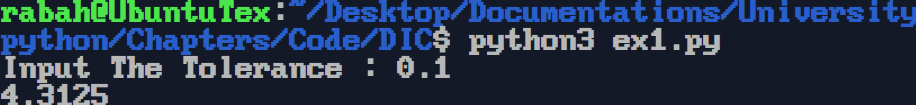
\includegraphics[width = 0.9\textwidth]{Chapters/ScreenShot/DIC/dic.png}
\end{center}

